\documentclass{beamer}
\usetheme{metropolis}
\usepackage{graphicx}
\usepackage{subfig}
\usepackage{hyperref}
\usepackage{tcolorbox}
\title{Algebra-Based Physics-1: Mechanics (PHYS135A-01): Week 6}
\date{October 9th - October 13th, 2017}
\author{Jordan Hanson}
\institute{Whittier College Department of Physics and Astronomy}

\begin{document}
\maketitle

\section{Week 5 Review}

\begin{frame}{Week 5 Review}
\begin{enumerate}
\item \alert{Friction}
\begin{itemize}
\item Normal force and friction
\item Static, kinetic
\end{itemize}
\item \alert{Drag}
\begin{itemize}
\item Terminal velocity
\end{itemize}
\item \alert{Restoring Forces}
\begin{itemize}
\item Hooke's Law
\item Young's modulus
\item Shear modulus
\item Bulk modulus
\end{itemize}
\end{enumerate}
\end{frame}

\section{Week 5 Review Problem}

\begin{frame}{Week 5 Review Problem}
A car rests on four shock absorbers, and each is like a spring with a spring constant $k = 1000 N/cm$.  The car weighs 10000 N.  By what distance is each spring compressed?
\begin{itemize}
\item A: 2.5 cm
\item B: 10 cm
\item C: 1 meter
\item D: 0 cm
\end{itemize}
\end{frame}

\begin{frame}{General Review Problem}
\begin{columns}[T]
\begin{column}{0.5\textwidth}
\small
Consider the 50.0 kg ice skater being pushed with $|\vec{F}_{\rm 1}|=|\vec{F}_{\rm 2}|=20.0$ N.  If her skates have a coefficient of kinetic friction of $\mu_{\rm k} = 0.02$, what is her acceleration?
\begin{itemize}
\item A: $3/5$ m s$^{-2}$, 45$^{\circ}$ from $\hat{i}$.
\item B: $(2\sqrt{2}-1)/5$ m s$^{-2}$, 45$^{\circ}$ from $\hat{i}$.
\item C: $(2\sqrt{2}-1)$ m s$^{-2}$, 45$^{\circ}$ from $\hat{i}$.
\item D: $3/5$ N, 45$^{\circ}$ from $\hat{i}$.
\end{itemize}
\end{column}
\begin{column}{0.5\textwidth}
\begin{figure}
\centering
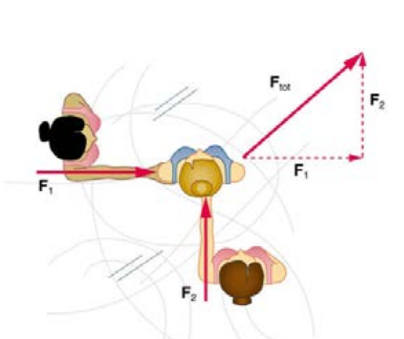
\includegraphics[width=0.7\textwidth]{figures/skate.png}
\caption{\label{fig:skate} Two skaters push a third.}
\end{figure}
\end{column}
\end{columns}
\end{frame}

\section{Week 6 Summary}

\begin{frame}{Week 6 Summary}
\begin{enumerate}
\item \alert{Angular} kinematics and dynamics
\begin{itemize}
\item Angular displacement
\item Angular velocity
\item Centripetal acceleration
\end{itemize}
\item \alert{Newton's Law of Gravity} and circular orbits
\item Kepler's Laws
\end{enumerate}
\end{frame}

\section{Angular Kinematics and Dynamics}

\begin{frame}{Angular Kinematics and Dynamics}
There is a correspondence between \alert{angular and linear kinetmatics}, if we deal with accelerations that are constant or zero.
\begin{columns}[T]
\begin{column}{0.5\textwidth}
\centering
\textbf{Linear}:
\begin{align}
x(t) &= x_{\rm 0} + v_{\rm i}t + \frac{1}{2}at^2 \\
v(t) &= v_{\rm i} + at \\
v^2 &= v_{\rm i}^2 + 2a(x-x_{\rm 0})
\end{align}
\end{column}
\begin{column}{0.5\textwidth}
\centering
\textbf{Angular}:
\begin{align}
\theta(t) &= \theta_{\rm 0} + \omega_{\rm i}t + \frac{1}{2}\alpha t^2 \\
\omega(t) &= \omega_{\rm i} + \alpha t \\
\omega^2 &= \omega_{\rm i}^2 + 2\alpha(\theta-\theta_{\rm 0})
\end{align}
\end{column}
\end{columns}
\end{frame}

\begin{frame}{Angular Kinematics and Dynamics}
\begin{figure}
\centering
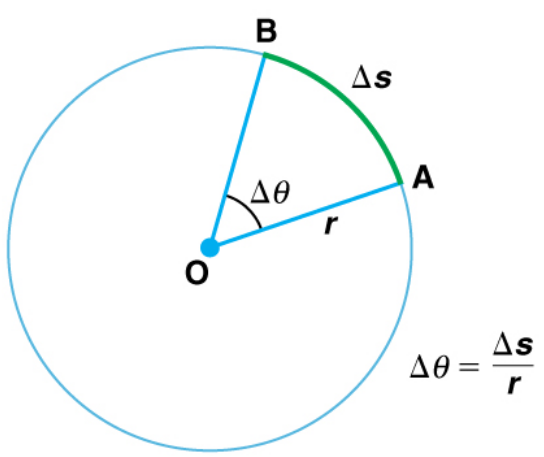
\includegraphics[width=0.6\textwidth]{figures/circle1.png}
\caption{\label{fig:circle1} The definitions of arc length, $\Delta s$, radius, r, and angular displacement $\Delta\theta$.}
\end{figure}
\end{frame}

\begin{frame}{Angular Kinematics and Dynamics}
\begin{columns}[T]
\begin{column}{0.5\textwidth}
\begin{figure}
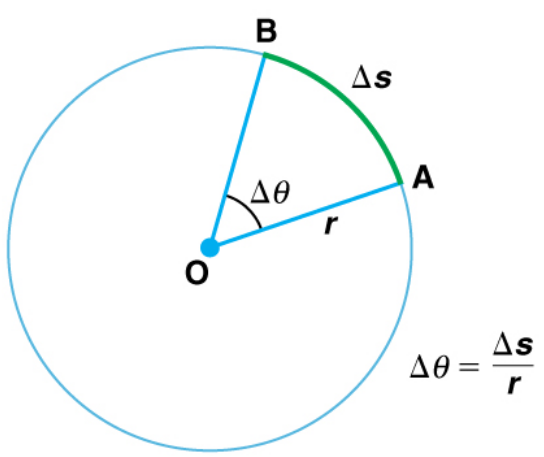
\includegraphics[width=0.6\textwidth]{figures/circle1.png}
\caption{\label{fig:circle2} \small Examining the change in these quantities: $\Delta\theta/\Delta t = \omega$, $\Delta\omega/\Delta t = \alpha$.}
\end{figure}
\end{column}
\begin{column}{0.5\textwidth}
\centering
Relationship between linear and rotational:
\begin{align}
v = \frac{\Delta s}{\Delta t} &= r \frac{\Delta\theta}{\Delta t} = r\omega \\
a = \frac{\Delta v}{\Delta t} &= r \frac{\Delta\omega}{\Delta t} = r\alpha
\end{align}
Notice that the units of angular velocity are s$^{-1}$, and those of angular acceleration are s$^{-2}$.
\end{column}
\end{columns}
\end{frame}

\begin{frame}{Angular Kinematics and Dynamics}
Astromers have now discovered several thousand planets orbiting in star systems other than ours.  Suppose we observe a star system face-on, and see a planet orbiting in a circular orbit with constant angular velocity.  If it goes halfway around the star in 3 months, what is the angular velocity of the planet?
\begin{itemize}
\item A: $\frac{\pi}{3}$ months$^{-1}$
\item B: $\frac{\pi}{6}$ months$^{-1}$
\item C: $\frac{2\pi}{3}$ months$^{-1}$
\item D: $2\pi$ months$^{-1}$
\end{itemize}
\end{frame}

\begin{frame}{Angular Kinematics and Dynamics}
If we define a coordinate system such that at time $t = 0$ months, the planet is along the x-axis, in how many months will the planet cross the negative y-axis?
\begin{itemize}
\item A: 3 months
\item B: 3.5 months
\item C: 4.0 months
\item D: 4.5 months
\end{itemize}
\end{frame}

\begin{frame}{Angular Kinematics and Dynamics}
\small
The lady-bug PheT: \\
\url{http://cnx.org/content/m42083/1.7/rotation_en.jar} \\ \vspace{0.5cm}
On a sheet of paper, make the following observations:
\begin{enumerate}
\item Measure the period of the motion of the lady-bug (x-y plot), and show that it is equal to the inverse of the frequency.  Write down your results.
\item Show that the tangential velocity of the lady-bug (v plot) is proportional to the radius of the lady-bug by plotting v versus radius.
\item Copy down the graph of $\theta(t)$, and measure $\omega$ from the $\omega$ plot.  Show that $\theta(t) = \theta_i + \omega t$ by plugging in several points from the graph into this formula.
\item When does $\theta(t) = \theta_i + \omega t$ not hold?  What is $\alpha$ in these cases?
\end{enumerate}
\end{frame}

\begin{frame}{Angular Kinematics and Dynamics}
\begin{columns}[T]
\begin{column}{0.5\textwidth}
\begin{figure}
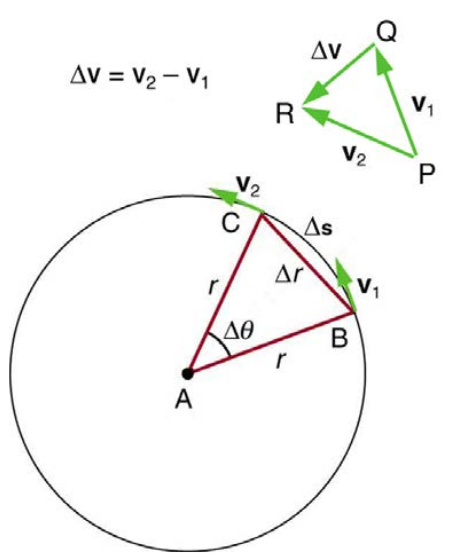
\includegraphics[width=0.6\textwidth]{figures/circle2.png}
\caption{\label{fig:circle3} \small The velocity triangle and the position triangle are \textit{similar}, because they are isosceles with the same angle ($\Delta\theta$).}
\end{figure}
\end{column}
\begin{column}{0.5\textwidth}
\centering
Similar triangles have equal \textit{ratios of sides}:
\begin{align}
\frac{\Delta v}{v} &= \frac{\Delta s}{r} \\
\Delta v &= \frac{v}{r}\Delta s \\
\frac{\Delta v}{\Delta t} &= \frac{v}{r}\frac{\Delta s}{\Delta t} \\
\Delta t &\to 0 \\
a_{\rm C} &= \frac{v^2}{r} = r \omega^2 \\
\vec{a}_{\rm C} &= - \frac{v^2}{r} \hat{r}
\end{align}
\end{column}
\end{columns}
\end{frame}

\begin{frame}{Angular Kinematics and Dynamics}
With centripetal acceleration comes \textbf{\alert{centripetal force}}, which is the net force for uniform circular motion:
\begin{equation}
\vec{F}_{\rm C} = - \frac{mv^2}{r}\hat{r} = -m r \omega^2 \hat{r}
\label{eq:centripetalForce}
\end{equation}
In Eq. \ref{eq:centripetalForce}, the minus sign indicates that the force points towards the center of the circle.
\end{frame}

\begin{frame}{Angular Kinematics and Dynamics}
\begin{columns}[T]
\begin{column}{0.45\textwidth}
\small
A liquid sample spins 7.50 cm from the axis of an centrifuge at $7.5 \times 10^2$ revolutions per minute.  What is this acceleration in g's?
\begin{itemize}
\item A: 46 g's
\item B: 460 g's
\item C: 1.2 g's
\item D: 12.0 g's
\end{itemize}
\end{column}
\begin{column}{0.55\textwidth}
\begin{figure}
\centering
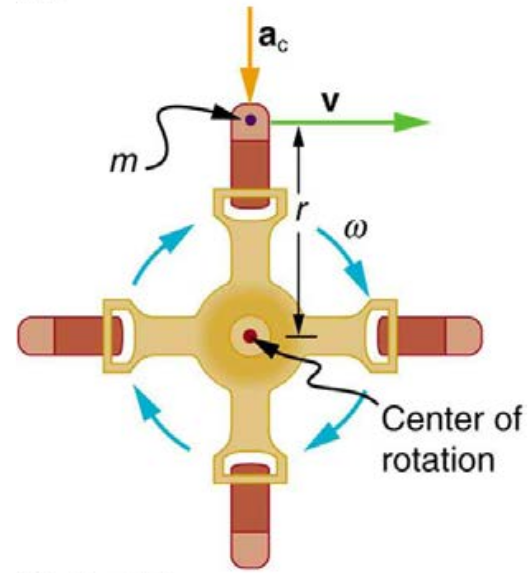
\includegraphics[width=0.9\textwidth]{figures/centrifuge.png}
\end{figure}
\end{column}
\end{columns}
\end{frame}

\begin{frame}{Angular Kinematics and Dynamics}
Calculate the centripetal force exerted on a 900 kg car that negotiates a 500 m radius curve at 25.0 m/s.
\begin{itemize}
\item A: 900 N
\item B: 9000 N
\item C: 1050 N
\item D: 1125 N
\end{itemize}
\end{frame}

\begin{frame}{Angular Kinematics and Dynamics}
What is the coefficient of friction required to keep the car from sliding?  (This is an example of \textit{static} fricion).
\begin{itemize}
\item A: 0.0
\item B: 0.1
\item C: 0.125
\item D: 0.25
\end{itemize}
\end{frame}

\begin{frame}{Angular Kinematics and Dynamics}
\begin{columns}[T]
\begin{column}{0.5\textwidth}
\begin{figure}
\centering
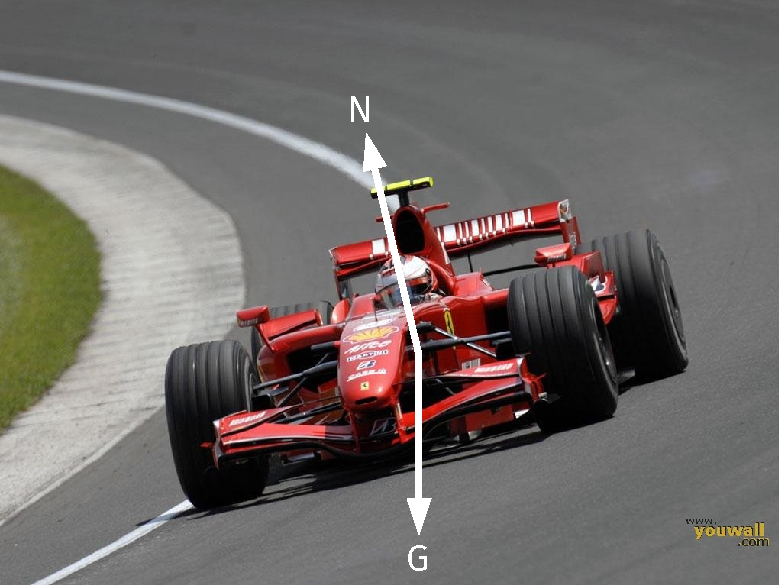
\includegraphics[width=0.9\textwidth]{figures/ferari.pdf}
\caption{\label{fig:ferari} There are two \alert{\textit{external}} forces on the automobile: normal force and weight.}
\end{figure}
\end{column}
\begin{column}{0.5\textwidth}
\small
Suppose the angle between the surface of a banked curve and horizontal is $\theta$.
\begin{align}
N\cos\theta &= mg \\
N\sin\theta &= m\frac{v^2}{r} \\
\frac{\sin\theta}{\cos\theta} &= \frac{v^2}{rg} \\
\tan\theta &= \frac{v^2}{rg}
\end{align}
Notice that centripetal force is not an \textit{external} force.
\end{column}
\end{columns}
\end{frame}

\begin{frame}{Angular Kinematics and Dynamics}
If the banked curve makes an angle of 30 degrees and has a radius of 500 meters, what is the maximum speed the F1 car may have? (Assume no friction).
\begin{itemize}
\item A: 54 m/s
\item B: 110 m/s
\item C: 10 m/s
\item D: 42 m/s
\end{itemize}
\end{frame}

\begin{frame}{Angular Kinematics and Dynamics - Extra Credit Problem}
\begin{columns}[T]
\begin{column}{0.5\textwidth}
\begin{figure}
\centering
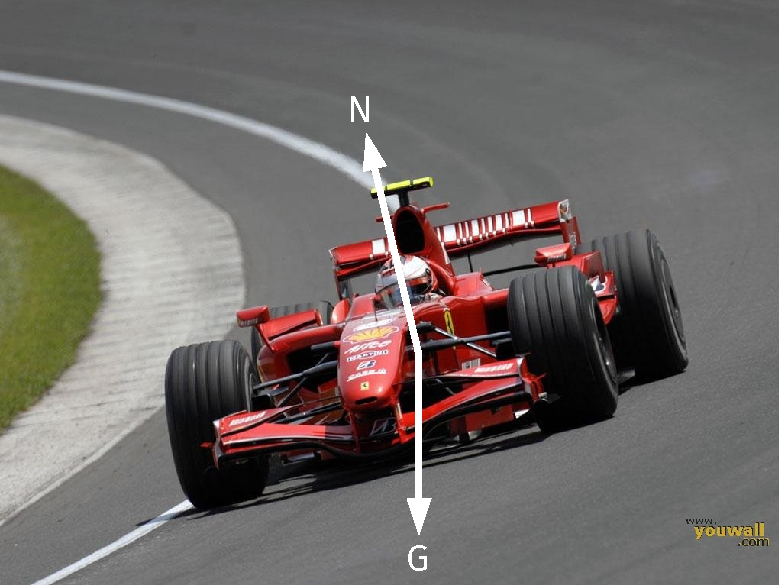
\includegraphics[width=0.9\textwidth]{figures/ferari.pdf}
\caption{\label{fig:ferari2} There are two \alert{\textit{external}} forces on the automobile: normal force and weight.}
\end{figure}
\end{column}
\begin{column}{0.5\textwidth}
\small
\textbf{Group activity}: Suppose the banked curve has a coefficient of static friction $\mu$, a radius $r$, and a bank angle $\theta$.  Show that the maximum velocity the F1 car may have without sliding is 
\begin{equation}
v = \sqrt{rg\left(\frac{\tan\theta+\mu}{1-\mu\tan\theta}\right)}
\end{equation}
\textbf{Google plotting}: Using Google, plot the term in parentheses versus $\theta$ for different fixed $\mu$-values, and discuss the differences in the shape of the curves.
\end{column}
\end{columns}
\end{frame}

\begin{frame}{Angular Kinematics and Dynamics}
\begin{columns}[T]
\begin{column}{0.5\textwidth}
\begin{figure}
\centering
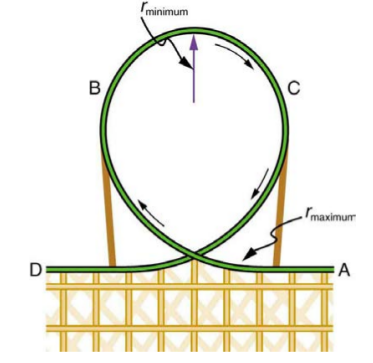
\includegraphics[width=0.9\textwidth]{figures/loop.png}
\caption{\label{fig:loop1} A loop in a roller coaster.}
\end{figure}
\end{column}
\begin{column}{0.5\textwidth}
\small
Notice that the radius of curvature in the roller coaster at left decreases.  Where will the centripetal force be highest?
\begin{itemize}
\item A: At left between A and B
\item B: At the top between B and C
\item C: At right between C and D
\item D: At the bottom
\end{itemize}
\end{column}
\end{columns}
\end{frame}

\begin{frame}{Angular Kinematics and Dynamics}
\begin{columns}[T]
\begin{column}{0.5\textwidth}
\begin{figure}
\centering
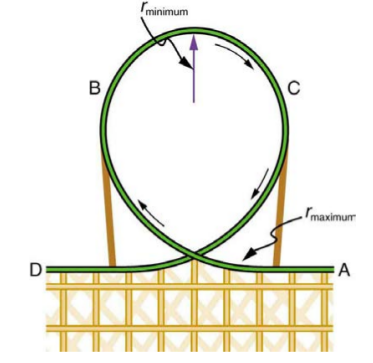
\includegraphics[width=0.9\textwidth]{figures/loop.png}
\caption{\label{fig:loop1} A loop in a roller coaster.}
\end{figure}
\end{column}
\begin{column}{0.5\textwidth}
\small
Suppose near the top, that $r = 40$ m and $v = 20$ m/s.  What is the centripetal acceleration?
\begin{itemize}
\item A: 1 m/s$^2$
\item B: 5 m/s$^2$
\item C: 10 m/s$^2$
\item D: 20 m/s$^2$
\end{itemize}
\end{column}
\end{columns}
\end{frame}

\section{Newton's Law of Gravity and Circular Orbits}

\begin{frame}{Newton's Law of Gravity and Circular Orbits}
\begin{figure}
\centering
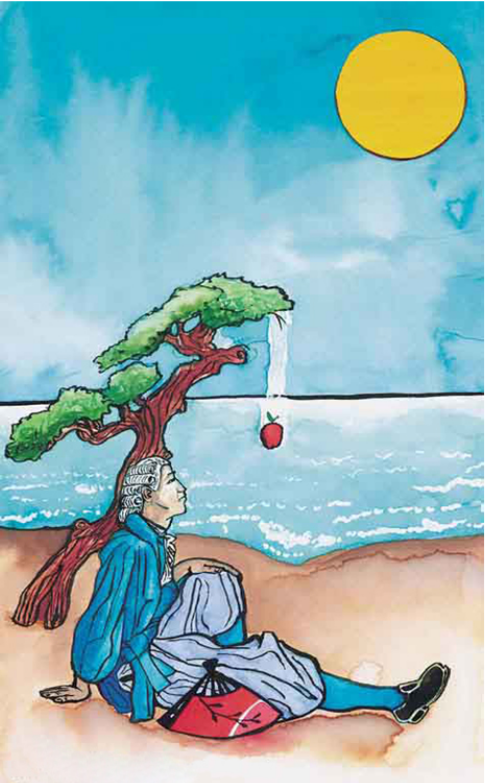
\includegraphics[width=0.35\textwidth]{figures/newton.png}
\caption{\label{fig:apple} Sir Isaac Newton realizing that the force between the ground and the tree could extend to the sun...}
\end{figure}
\end{frame}

\begin{frame}{Newton's Law of Gravity and Circular Orbits}
\begin{figure}
\centering
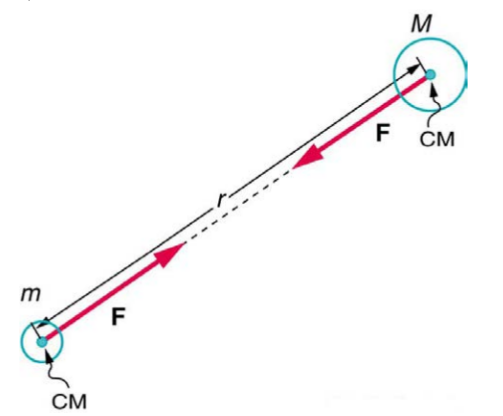
\includegraphics[width=0.55\textwidth]{figures/third.png}
\caption{\label{fig:third} Remember: the force of gravity must obey Newton's Third Law, like any other force.}
\end{figure}
\end{frame}

\begin{frame}{Newton's Law of Gravity and Circular Orbits}
Gravity PheT: \\
\url{http://cnx.org/content/m42086/1.9/gravity-and-orbits_en.jar}
\begin{enumerate}
\item Begin an orbit of the Earth around the Sun.  What happens when you change the mass of either object?
\item Are the forces of gravity on the objects ever unequal?  What does Newton's Third Law tell you?
\item What is the relationship between the period and the orbital radius (qualitatively)?
\end{enumerate}
\end{frame}

\begin{frame}{Newton's Law of Gravity and Circular Orbits}
\begin{tcolorbox}[colback=white,colframe=red!40!blue,title=Newton's Law of Gravitation]
\alert{Let two systems have masses $m_1$ and $m_2$, the distance between them be $r$, and $G = 6.674\times 10^{-11}$ N m$^2$ kg$^{-2}$.  The force of gravity between them is}\vspace{0.2cm}
\alert{$\vec{F} = G\frac{m_1 m_2}{r^2}\hat{r}$}
\end{tcolorbox}
\end{frame}

\begin{frame}{Newton's Law of Gravity and Circular Orbits}
The radius of the Earth is $6.38\times 10^6$ m, the mass of the Earth is $5.98 \times 10^{24}$ kg, and $G = 6.674\times 10^{-11}$ N m$^2$ kg$^{-2}$.  Using Newton's Second Law and Newton's Law of Gravity, show that the acceleration of systems with mass $m$ at the radius of the Earth is $\approx 9.8$ m/s$^2$.\\
\vspace{0.2cm}
(Set $F_{\rm Net} = G\frac{Mm}{r^2}$, where M is the mass of the Earth).
\end{frame}

\begin{frame}{Newton's Law of Gravity and Circular Orbits}
What is the period of the moon's orbit around the Earth?  Start by setting gravitational force equal to the centripetal force.  (Earth-moon distance is $3.84\times 10^8$ m, mass of the Earth is $5.98 \times 10^{24}$ kg, and $G = 6.674\times 10^{-11}$ N m$^2$ kg$^{-2}$).
\begin{itemize}
\item A: 25.5 days
\item B: 27.4 days
\item C: 29.1 days
\item D: 31.0 days
\end{itemize}
\end{frame}

\begin{frame}{Newton's Law of Gravity and Circular Orbits}
\textbf{Orbital velocity}: What is the speed of the International Space Station in orbit around the Earth?  (Assume it is orbiting at the radius of the Earth).
\begin{itemize}
\item A: 100 m/s
\item B: 1 km/s
\item C: 10 km/s
\item D: 100 km/hr
\end{itemize}
\end{frame}

\section{Kepler's Laws and Newton's Laws of Gravity}

\begin{frame}{Kepler's Laws and Newton's Laws of Gravity}
The development of the law of gravitation played a ``pivotal role in the history of ideas,'' according to the text.  One simple observation and the ensuing analysis led to explanations for: \\
\begin{itemize}
\item The orbit of the moon
\item The tides
\item The \alert{heliocentric universe}
\item The orbits of planets, including Kepler's Laws
\item Comets (not always in orbit)
\item The story of Edmond Halley, and measuring 1 AU in meters
\item How to get to Mars
\item All the things
\end{itemize}
\end{frame}

\begin{frame}{Kepler's Laws and Newton's Laws of Gravity}
Kepler's first law: \\
\vspace{0.5cm}
\textbf{The orbit of each planet about the Sun is an ellipse with the Sun at one focus.} \\
\vspace{0.5cm}
The approximation of circular orbits holds when one system is much more massive than the other, and there are no perturbations from other orbiting systems.
\end{frame}

\begin{frame}{Kepler's Laws and Newton's Laws of Gravity}
\begin{figure}
\centering
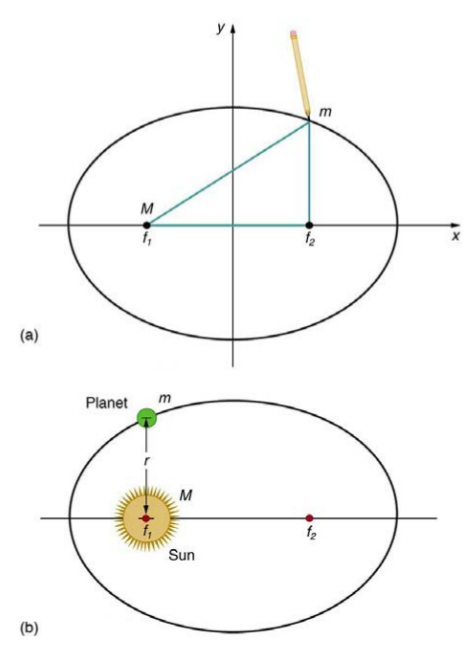
\includegraphics[width=0.4\textwidth]{figures/kepler1.png}
\caption{\label{fig:kepler1} Diagram of Kepler's first law.  The ellipse does not have a center and a radius, but two \textit{focii} and a radius that varies.}
\end{figure}
\end{frame}

\begin{frame}{Kepler's Laws and Newton's Laws of Gravity}
Kepler's second law: \\
\vspace{0.5cm}
\textbf{Each planet moves so that an imaginary line drawn from the Sun to the planet sweeps out equal areas in equal times.} \\
\vspace{0.5cm}
This rule accounts for the fact that the centripetal acceleration increases if the radius (which can vary) decreases.  That means that when the orbiting system is closer to more massive system, the orbital velocity must increase.
\end{frame}

\begin{frame}{Kepler's Laws and Newton's Laws of Gravity}
\begin{figure}
\centering
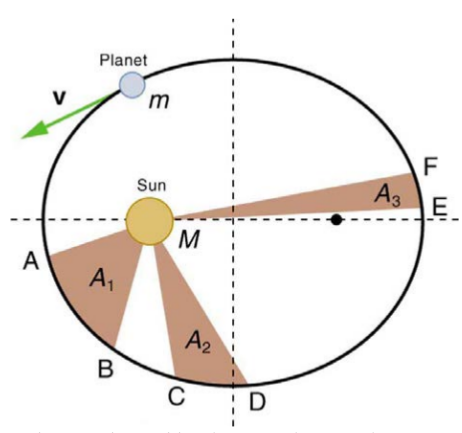
\includegraphics[width=0.6\textwidth]{figures/kepler2.png}
\caption{\label{fig:kepler2} Diagram of Kepler's second law.  Each shaded area has equal area, and corresponds to equal time, but not equal orbital distance.}
\end{figure}
\end{frame}

\begin{frame}{Kepler's Laws and Newton's Laws of Gravity}
Kepler's third law: \\
\vspace{0.5cm}
\textbf{The product of the orbital period squared and the orbital radius cubed of the orbiting system remains constant.} \\
\vspace{0.5cm}
We can derive this fact from Newton's Law of Gravity...
\end{frame}

\begin{frame}{Kepler's Laws and Newton's Laws of Gravity}
\textbf{Group activity}: Setting the law of gravity equal to the centripetal force, show that
\begin{equation}
\frac{r^3}{T^2} = \frac{GM}{4\pi^2}
\end{equation}
G is the gravity constant, and $M$ is the mass of the system being orbited.  \textit{Notice that the right-hand side is a constant.}  This implies that ratios of radii cubed and period squared should never change.
\end{frame}

\begin{frame}{Kepler's Laws and Newton's Laws of Gravity}
\begin{figure}
\centering
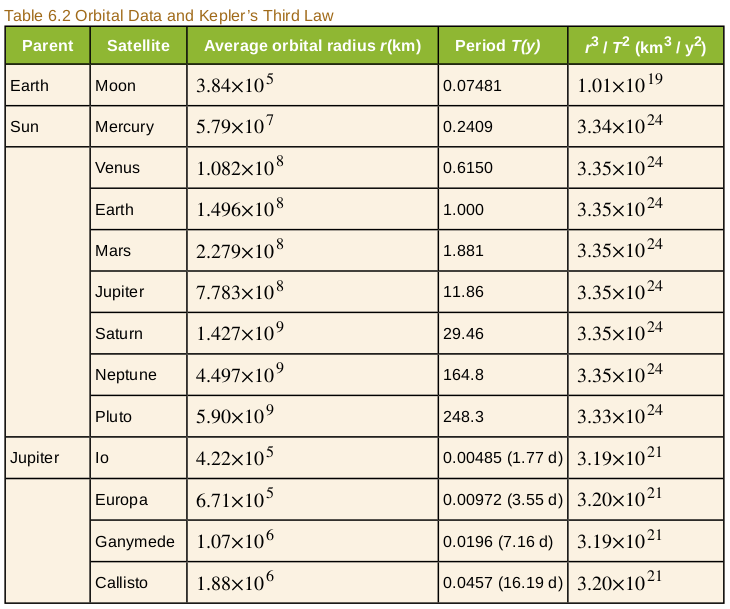
\includegraphics[width=0.6\textwidth]{figures/keplertable.png}
\caption{\label{fig:kepler3} Kepler and his advisor Brache collected data such as this, and determined empirically the third law \textit{before} Sir Isaac Newton published the law of gravity.}
\end{figure}
\end{frame}

\begin{frame}{Kepler's Laws and Newton's Laws of Gravity}
\alert{Star party}: In late November we will be heading to the desert, and bringing telescopes to observe objects in the solar system and beyond!  Talk to me or Professor Piner about joining us... \\ \vspace{0.5cm}
\alert{+1 B.P. if you present what we discover in front of the class.}
\\ \vspace{0.5cm}
\textbf{Also a good final project: measuring the motion of a planet for several nights and explaining its motion.}
\end{frame}

\section{Conclusion}

\begin{frame}{Week 6 Summary}
\begin{enumerate}
\item \alert{Angular} kinematics
\begin{itemize}
\item Angular displacement
\item Angular velocity
\item Centripetal acceleration
\end{itemize}
\item \alert{Newton's Law of Gravity} and circular orbits
\item Kepler's Laws
\end{enumerate}
\end{frame}

\section{Answers}

\begin{frame}{Answers}
\begin{columns}[T]
\begin{column}{0.5\textwidth}
\begin{itemize}
\item 2.5 cm
\item $(2\sqrt{2}-1)/5$ m s$^{-2}$, 45$^{\circ}$ from $\hat{i}$.
\item $\frac{\pi}{3}$ months$^{-1}$
\item 4.5 months
\item 46 g's
\item 1125 N
\item 0.125
\item 54 m/s
\item At the top between B and C
\item 10 m/s$^2$
\item 27.4 days
\end{itemize}
\end{column}
\begin{column}{0.5\textwidth}
\begin{itemize}
\item 10 km/s 
\end{itemize}
\end{column}
\end{columns}
\end{frame}

\end{document}
